\chapter{Bogolon-mediated electron scattering in hybrid Bose--Fermi systems}\label{Ch6}
%
% ----------------------------------------------------------
%
In this chapter, we discuss the second topic of this thesis.
We show that when a 2D electron gas is coupled with a condensate of, e.g. indirect excitons, the contribution to the electron resistivity from the interaction with the excitations above the condensate can be orders of magnitude higher than the typical phonon contribution.
\section{Background}
Electron scattering in solid-state nanostructures plays a crucial role in their 2D transport~\cite{Kawamura:1992aa,Hwang:2008aa}, dramatically modifying electric conductivity.
%
Conventionally, there are two principal electron scattering mechanisms: disorder- or impurity-mediated~\cite{Jena:2007aa,Gibbons:2009aa}, and lattice phonon-mediated~\cite{Kawamura:1992aa}. The former processes are more pronounced at low environmental temperatures.
%
In the case of an attracting impurity, electrons can be captured, and thus the number of electrons decreases. Otherwise, repulsive centers decrease the electron mean free path and scattering time~\cite{Shi:2012aa,Bourgoin:1992aa,Eshchenko:2002aa,Palma:1995aa,Boev:2018ab}.
%
With an increase of temperature, electron scattering accompanied by acoustic and optical phonons of the crystal lattice becomes more efficient~\cite{Gummel:1955aa, Lax:1960aa, Abakumov:1976aa} and at some point dominant.

Conventional scattering mechanisms are also present in various new hybrid structures, which are the focus of current research~\cite{Cotlet:2016aa,Laussy:2010aa,Sau:2010aa,Alicea:2010aa,Mourik:2012aa}.
Hybrid Bose--Fermi systems represent a layer of fermions, usually a 2D electron gas (2DEG), coupled to another layer or layers of bosons such as excitons, exciton-polaritons, and Cooper pairs in superconductors.
% Hybrid systems consist of two-dimensional spatially separated layers, containing electrons in a two-dimensional electron gas (2DEG) phase and bosons, such as direct and indirect (dipolar) excitons, exciton polaritons, or the Cooper pairs in superconductors~\cite{Villegas:2018aa}.
In these systems, research interests are two-fold. One is devoted to high-temperature boson-mediated  superconductivity~\cite{Skopelitis:2018aa} and other condensation phenomena in interacting structures, including the Mott phase transition from an ordered state to electron-hole plasma~\cite{Kochereshko:2016aa}.
The other is devoted to finding additional new mechanisms of fermion scattering in the 2DEG, thus modifying the temperature dependence of the kinetic coefficients. Such possibilities explain the motivation to study electron transport in hybrid systems.

In this chapter, we will consider two different systems of fermion layers, specifically a layer of graphene (electrons with linear dispersion) and a layer of normal metal (electrons with parabolic dispersion).
Boson layers in both of the systems are expected as a condensed exciton gas, and the interactions between boson and fermion layers are described by Coulomb forces~\cite{Boev:2018ab,Kochereshko:2016aa, Matuszewski:2012aa}.
When the boson gas is in a condensed state, the corresponding interaction can be regarded as a counterpart to phonon-mediated scattering~\cite{Kovalev:2011aa, Kovalev:2013aa, Batyev:2014aa}.
% In this article, we show that in hybrid Bose-Fermi systems, which consist of spatially separated 2DEG in graphene layer and an exciton gas, interacting via the Coulomb forces~\cite{Boev:2016aa,Kochereshko:2016aa, Matuszewski:2012aa}, there appears a counterpart to the phonon-mediated scattering, when the gas of bosons is condensed~\cite{Kovalev:2011aa, Kovalev:2013aa, Batyev:2014aa}.
Such 2D condensation has been reported in various solid-state systems~\cite{Butov:2003aa,Kasprzak:2006aa,Schneider:2013aa},
%
in which the lattice vibrations turn out to be not the only \textit{sound} available.
In the presence of BEC~\cite{Butov:2003aa}, other excitations come into play, commonly referred to as Bogoliubov quasi-particles or bogolons, which have linear dispersion at small momenta.

In the following sections, we show that an additional principal mechanism of electron scattering appears, stemming from the inter-layer electron--exciton interaction, or bogolon-mediated scattering.
Also, we demonstrate that the difference between acoustic phonon-related and bogolon-assisted scattering is more than just the magnitude of the sound velocity.
%
% In graphene case, the dependence of the bogolon--mediated resistivity on temperature is $\sim T^4$ at low temperatures and $\sim T$ in the high-temperature limit.
% The dependence of the bogolon--mediated resistivity of graphene on temperature is $\sim T^4$ at low temperatures and $\sim T$ in the high-temperature limit.
% In contrasts, a precise calculation of the acoustic phonon--mediated resistivity in graphene shows $\rho\propto T^\alpha$ at low temperatures with $\alpha\sim6$~\cite{Kaasbjerg:2012aa}.
% Moreover, the phonon-mediated scattering is vulnerable to the screening effects~\cite{Hwang:2007aa}.
% This makes a great deal of difference between the two mechanisms of scattering, and one can surpass the other.

% For the case of the normal metal,

%
% ---------------------------------------
%
\section{System schematic}
Let us first consider a hybrid system consisting of a fermion layer separated by distance $l$ from a double QW that contains a dipolar exciton gas, where the distance between the layers of electrons and holes is $d$ (see Fig.~\ref{fig:Ch6_1}).
%
%
%
\begin{figure}[ht]
\centering
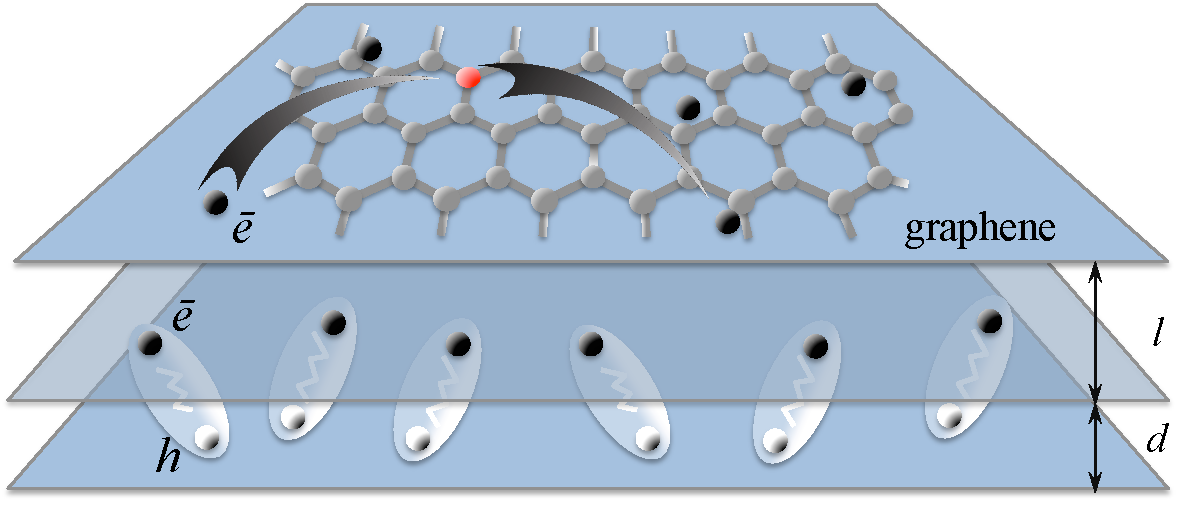
\includegraphics[width=0.69\textwidth]{Fig/Ch6/Fig1.pdf}
\caption[Hybrid system schematic]{System schematic. A fermion layer (here, graphene) is located at distance $l$ from a 2D dipolar exciton gas residing in two parallel layers at distance $d$ from each other. Particles couple via Coulomb interaction. The figure is taken from~\cite{Sun:2019aa}.}
\label{fig:Ch6_1}
\end{figure}
%
%
%
Electron--exciton interaction in this system can be described by the Hamiltonian
%
\begin{equation}\label{CH6_eq.1}
V=\int d\mathbf{r}\int d\mathbf{R}\Psi^\dag_\mathbf{r}\Psi_\mathbf{r}g\left(\mathbf{r}-\mathbf{R}\right)\Phi^\dag_\mathbf{R}\Phi_\mathbf{R},
\end{equation}
%
where $\Psi_\mathbf{r}$ and $\Phi_\mathbf{R}$ are the quantum field operators of the electrons and excitons, respectively, $g\left(\mathbf{r}-\mathbf{R}\right)$ is the Coulomb interaction between an electron and an exciton, $\mathbf{r}$ is the electron coordinate within the fermion layer, and $\mathbf{R}$ is the exciton center-of-mass coordinate.
We disregard the internal structure of the excitons to focus on their collective motion.

We assume that the temperature of the system is below the critical temperature at which the excitons become a degenerate Bose gas~\cite{Fogler:2014aa}. This temperature is given by $kT_c =\frac{2\pi\hbar^2}{m_x}n_x$, where $n_x$ and $m_x$ are the exciton density and effective mass, respectively.
We can then use the model of a weakly interacting non-ideal Bose gas and write the exciton field operators as $\Phi_\mathbf{R}=\sqrt{n_c}+\phi_\mathbf{R}$, where $n_c$ is the condensate density.
In other words, we separate the condensed and non-condensed particles.
%
Substituting this into Eq.~\eqref{CH6_eq.1} and taking into account the selection rules, we find the electron--bogolon interaction potential by
%
\begin{eqnarray}
V_1 &=& \sqrt{n_c}\int d\mathbf{r}\Psi^\dag_\mathbf{r}\Psi_\mathbf{r} \int d\mathbf{R}g\left(\mathbf{r}-\mathbf{R}\right)\left[\varphi^\dag_\mathbf{R}+\varphi_\mathbf{R}\right],\label{CH6_eq.2-a} \\
V_2 &=& \int d\mathbf{r} \Psi^\dagger_\mathbf{r} \Psi_\mathbf{r} \int d\mathbf{R} g\left(\mathbf{r}-\mathbf{R}\right) \phi^\dagger_\mathbf{R} \phi_\mathbf{R}. \label{CH6_eq.2-b}
\end{eqnarray}
%
Furthermore, we take the Fourier transform of the operators in Eq.~\eqref{CH6_eq.2-a} and Eq.~\eqref{CH6_eq.2-b}, using
%
\begin{equation}\label{CH6_eq.3}
    \varphi^\dag_\mathbf{R}+\varphi_\mathbf{R}= \frac{1}{L}\sum_{\mathbf{p}} e^{\mi\mathbf{pR}} \left[(u_\mathbf{p}+v_{-\mathbf{p}})b_\mathbf{p}+(v_\mathbf{p}+u_{-\mathbf{p}})b^\dag_{-\mathbf{p}}\right],
\end{equation}
%
where $b^\dag_{\mathbf{p}}$ and $b_{\mathbf{p}}$ are the creation and annihilation operators of the bogolons, respectively, with the coefficients reading~\cite{Giorgini:1998aa}
%
\begin{eqnarray}\label{CH6_eq.4}
    u^2_{\mathbf{p}}=1+v^2_{\mathbf{p}}&=&\frac{1}{2}\left(1+\left[1+\frac{(Ms^2)^2}{\omega^2_{\mathbf{p}}}\right]^{1/2}\right),\\\nonumber
    u_{\mathbf{p}}v_{\mathbf{p}}&=&-\frac{Ms^2}{2\omega_{\mathbf{p}}}.
\end{eqnarray}
%
Here $M$ is the exciton mass, $s=\sqrt{\kappa n_c/M}$ is the sound velocity of the bogolons,
$\omega_k=sk(1+k^2\xi^2)^{1/2}$ is their spectrum, $\kappa=e_0^2d/\epsilon$ is the Fourier image of the exciton--exciton interaction strength, $e_0$ is electron charge, $\epsilon$ is the dielectric function, and $\xi=\hbar/(2Ms)$ is the healing length of the condensation.
%
Combining Eqs.~\eqref{CH6_eq.2-a}--\eqref{CH6_eq.3} with the Fourier transformation of operator for electron $\Psi_\mathbf{r}=\frac{1}{L}\sum_\mathbf{k} c_\mathbf{k} e^{\mi\mathbf{k}\mathbf{r}}$ yields
%
\begin{eqnarray}
V_1 &=& \frac{\sqrt{n_c}}{L} \sum_{\mathbf{k,p}} g_\mathbf{p} \left[ \left( v_\mathbf{p} + u_\mathbf{-p} \right)b^\dagger_\mathbf{-p} + \left( u_\mathbf{p} + v_\mathbf{-p}\right)b_\mathbf{p} \right] c^\dagger_\mathbf{k+p} c_\mathbf{k}, \label{CH6_eq.5-a} \\
V_2 &=& \frac{1}{L^2}\sum_{\mathbf{k},\mathbf{p},\mathbf{q}} g_\mathbf{p}\bigg[ u_{\mathbf{q}-\mathbf{p}} u_\mathbf{q} b^\dagger_{\mathbf{q}-\mathbf{p}} b_\mathbf{q} + u_{\mathbf{q}-\mathbf{p}} v_\mathbf{q} b^\dagger_{\mathbf{q}-\mathbf{p}} b^\dagger_{-\mathbf{q}} \nonumber \\
&+& v_{\mathbf{q}-\mathbf{p}} u_\mathbf{q} b_{-\mathbf{q}+\mathbf{p}} b_\mathbf{q} + v_{\mathbf{q}-\mathbf{p}} v_\mathbf{q} b_{-\mathbf{q}+\mathbf{p}} b^\dagger_{-\mathbf{q}}\bigg] c^\dagger_{\mathbf{k}+\mathbf{p}} c_\mathbf{k},\label{CH6_eq.5-b}
\end{eqnarray}
%
where $g_\mathbf{p}$ is the Fourier image of the electron--exciton interaction, which we will discuss in a later section, and $L$ is the size of the system.
%
Illustrations of the processes in Eqs.~\eqref{CH6_eq.5-a} and ~\eqref{CH6_eq.5-b} are presented in Fig.~\ref{fig:CH6_2}, which depicts the scattering of an electron mediated by the absorption or emission of bogolons.
%
%
%
\begin{figure}[ht]
    \centering
    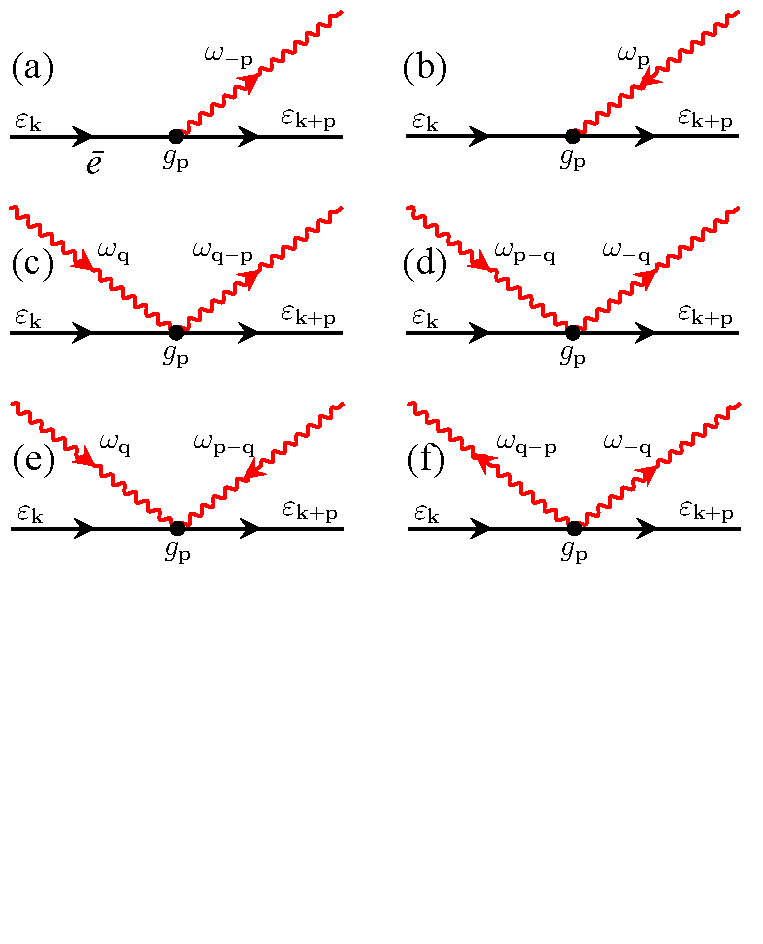
\includegraphics[width=0.60\textwidth]{Fig/Ch6/Fig2.pdf}
    \caption[Electron scattering diagrams]{Schematic of electron scattering as mediated by bogolon emission and absorption processes. The black lines represent the electrons and the red wavy lines are the bogolons. (a,b) Single-bogolon scattering events from Eq.~\eqref{CH6_eq.5-a}. (c--f) Double-bogolon scattering events from Eq.~\eqref{CH6_eq.5-b}. The figure is taken from~\cite{Villegas:2019aa}.}
    \label{fig:CH6_2}
\end{figure}
%
%
%

\section{Electron--exciton interaction}
To derive the formula of the interaction term in momentum space, we consider the system as shown in Fig.~\ref{fig:CH6_gk}.
%
\begin{figure}
    \centering
    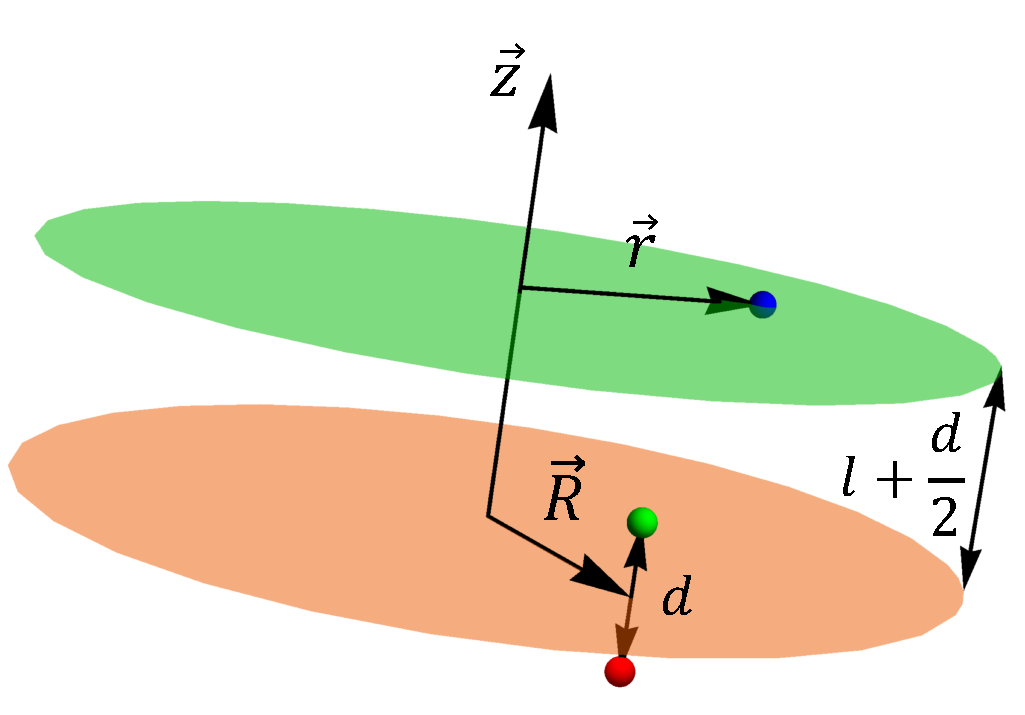
\includegraphics[width=0.55\textwidth]{Fig/Ch6/elec-exc.pdf}
    \caption[Electron and exciton interaction in the hybrid system]{Schematic of the interaction between an electron and exciton (electron--hole pair) in the hybrid system. The blue dot in the green disk is an electron with coordinate $\mathbf{r}$ in the fermion layer. For the exciton, we consider the center of mass for the electron--hole pair, labeled by $\mathbf{R}$ in the orange plane. The green (red) dot represents the electron (hole) of the exciton. As shown in Fig.~\ref{fig:Ch6_1}, parameters $l$ and $d$ are the distances between layers in the $z$-direction. Assuming the effective mass of the electron and hole is the same, then the distance between the green and orange planes is $l+\frac{d}{2}$.  }
    \label{fig:CH6_gk}
\end{figure}
%
The electron located in the fermion layer is represented by the blue dot in the green disk.
Vector $\mathbf{r}$ represents the location of the electron in the fermion layer, where the origin is the point where the $z$-axis intersects with the green plane.
For the exciton, we consider the center of mass represented by $\mathbf{R}$ in the orange disk.

By the notations $r_{e-e}$ ($r_{e-h}$) representing the distance between electron--electron (electron--hole), $e_0$ representing the unit of electron charge and $\epsilon$ representing the dielectric constant for the given material, considering the formula of Coulomb potential we have
%
\begin{eqnarray}
g\left(r\right) &=& \frac{e_0^2}{4\pi\epsilon}\left( \frac{1}{r_{e-e}}-\frac{1}{r_{e-h}}\right) \\ \nonumber
&=& \frac{e_0^2}{4\pi \epsilon} \left( \frac{1}{\sqrt{l^2+\left( \mathbf{r} - \mathbf{R} \right)^2}} - \frac{1}{\sqrt{ \left(l+d\right)^2+\left( \mathbf{r} -\mathbf{R} \right)^2 }}\right), \label{eq:CH6_gk_real_space}
\end{eqnarray}
where, as shown in Fig.~\ref{fig:CH6_gk}, the 2D vectors $\mathbf{r}$ and $\mathbf{R}$ are the positions of the electron and exciton in their respective layers, and $l$ and $d$ are the distances in the $z$-direction between layers.

Renewing the variable $\mathbf{r}$ by the definition $\mathbf{r} \equiv \mathbf{r} - \mathbf{R}$ and then applying the Fourier transform, we have
\begin{eqnarray}
 g\left( \mathbf{k} \right) &=& \frac{e_0^2}{4\pi \epsilon} \int d\mathbf{r} \left[ \left( l^2 + \mathbf{r}^2 \right)^{-\frac{1}{2}} -\left( \left( l+d \right)^2 + \mathbf{r}^2 \right)^{-\frac{1}{2}} \right] e^{-\mi \mathbf{k} \cdot \mathbf{r}} \\ \nonumber
 &=& \frac{e_0^2}{4 \pi \epsilon} \int_0^\infty dr \int_0^{2\pi} d\theta \left[ \frac{re^{-\mi k r \cos\theta}}{\sqrt{l^2 + r^2}} - \frac{re^{-\mi k r \cos\theta}}{\sqrt{\left( l + d \right)^2 +r^2 }} \right] \\ \nonumber
 &=& \frac{e_0^2}{4 \pi \epsilon} \int_0^\infty dr \left[ \frac{r}{\sqrt{l^2 + r^2}} \frac{r}{\sqrt{\left( l+d \right)^2 + r^2}}\right] 2\pi \mathcal{J}_0\left( k r \right) \\ \nonumber
 &=& \frac{e_0^2}{2 k \epsilon } e^{-kl} \left( 1 - e^{-kd} \right),
\end{eqnarray}
where $\mathcal{J}_0$ is the Bessel function of first kind, and $k$ is the magnitude of $\mathbf{k}$.
We can further approximate this interaction by,
\begin{equation}
    g\left(\mathbf{k}\right) = \frac{e_0^2}{2k \epsilon}e^{-kl}.
    \label{eq:CH6_gk_k}
\end{equation}
We will use this formula in later calculations.
%
%
% -------------------------------------
%
\section{Graphene case}
In the graphene case, we will discuss the single-bogolon scattering process as described by Eq.~\eqref{CH6_eq.5-a}.
%We will not discuss two-bogolons scatter process in this thesis.
\subsection{Particle transport}
We use the Boltzmann transport theory \cite{Kawamura:1990aa} to calculate the resistivity of electrons in graphene, which is given by
%
\begin{equation}\label{CH6_eq.6}
\rho^{-1} = e_0^2 D\left(E_F\right)\frac{v_F^2}{2}\langle \tau \rangle,
\end{equation}
%
where $v_F$ is the Fermi velocity, $E_F$ is the Fermi energy, and the density of states of graphene at the Fermi level reads $D\left(E_F\right) =\left(g_s g_v/2\pi \hbar^2\right)E_Fv_F^{-2}$, where $g_{s,v}=2$ are the spin and valley $g$-factors, respectively.
%
We can write the energy-averaged relaxation time as~\cite{Kawamura:1990aa,PhysRevB.45.3612,Hwang:2008aa}
%
\begin{equation}\label{CH6_eq.7}
\langle \tau \rangle = \frac{\int d \varepsilon D\left(\varepsilon \right) \tau\left( \varepsilon \right) \left[ -\frac{df^0\left(\varepsilon\right)}{d \varepsilon}\right]}{\int d \varepsilon D\left(\varepsilon\right) \left[ -\frac{df^0\left(\varepsilon\right)}{d \varepsilon} \right]},
\end{equation}
%
where $f^0\left(\varepsilon\right)=\{\exp[(\varepsilon-\mu)/(k_BT)]+1\}^{-1}$ is the Fermi distribution function, $\mu$ is the chemical potential, $k_B$ is the Boltzmann constant, and the energy-dependent inverse relaxation time reads
%
\begin{equation}\label{CH6_eq.8}
  \frac{1}{\tau\left(\varepsilon\right)} = \sum_\mathbf{k'}\left(1 -\cos\theta_\mathbf{kk'}\right) W_\mathbf{kk'} \frac{1-f^0\left(\varepsilon'\right)}{1-f^0\left(\varepsilon\right)}.
\end{equation}
%
Here, $\theta_\mathbf{kk'}$ is the scattering angle between $\mathbf{k}$ and $\mathbf{k'}$, $\varepsilon=\hbar v_F\abs{\mathbf{k}}$ is the dispersion of graphene, and $W_\mathbf{kk'}$ is the probability of transition from an initial electron state $\mathbf{k}$ to the final state $\mathbf{k}'$, as given by
%
\begin{equation}\label{CH6_eq.9}
    W_\mathbf{kk'}=\frac{2\pi}{\hbar}\sum_\mathbf{q} \abs{C_\mathbf{q}}^2 \Delta\left(\varepsilon, \varepsilon'\right),
\end{equation}
%
where $C_\mathbf{q}$ is the scattering matrix element, and
%
\begin{equation}\label{CH6_eq.10}
  \Delta\left(\varepsilon,\varepsilon'\right)=N_q\delta\left(\varepsilon-\varepsilon'+\hbar\omega_q\right)+\left(N_q+1\right)\delta\left(\varepsilon-\varepsilon'-\hbar\omega_q\right),
\end{equation}
%
where $N_q=\{\exp[\hbar\omega_q/(k_BT)]-1\}^{-1}$ is the Bose distribution function.
%
Summing up, the energy-dependent relaxation time reads
%
\begin{eqnarray}\label{CH6_eq.11}
\frac{1}{\tau\left(\varepsilon\right)} &=& \frac{e_0^4 d^2 n_c}{8 \pi\epsilon^2 \hbar} \int d \mathbf{k'}\left(1-\cos\theta_{\mathbf{kk'}}\right) \int d \mathbf{q} e^{-2\abs{q}l}\abs{u_\mathbf{q}+v_\mathbf{q}}^2 \nonumber \\
&\times& \frac{1-f^0\left(\varepsilon'\right)}{1-f^0\left(\varepsilon\right)}\Delta\left(\varepsilon,\varepsilon'\right)\delta \left(\mathbf{q}-\mathbf{k}+\mathbf{k'}\right).
\end{eqnarray}
%
Using Eq.~\eqref{CH6_eq.4} and assuming a linear dispersion of bogolons $\omega_\mathbf{q}=s\abs{\mathbf{q}}$ (which is legitimate at $q\ll \xi^{-1}$ ), we find:
%
\begin{eqnarray} \label{CH6_eq.12}
\frac{1}{\tau\left(\varepsilon\right)} &=& \sum_{n=1,2}\frac{e_0^4 d^2 n_c }{8\pi \epsilon^2 \hbar^3 v_F^2} \int_0^{2\pi} d\theta \varepsilon_n \left( 1-\cos\theta\right)  \frac{1-f^0\left(\varepsilon_n \right) } {1-f^0\left(\varepsilon\right)} \nonumber \\ 
&\times& e^{-2l\lambda}\left( \sqrt{1+\frac{M^2s^2}{\hbar^2\lambda^2}} - \frac{Ms}{\hbar \lambda}\right) \frac{N_\lambda + \delta_{n,2}}{|F'_n \left( \varepsilon_n \right) |} ,
\end{eqnarray}
%
where $\lambda\equiv\abs{\mathbf{k}-\mathbf{k'}} = \sqrt{k^2+k'^2-2kk'\cos\theta}$ and thus is a function of $k$, $k'$, and $\theta$, $\varepsilon_n$ are two roots of the equation $F_{1,2} \left(\varepsilon'\right)=\varepsilon-\varepsilon'\pm \hbar \omega_\lambda=0$, $F'_{n}\left(\varepsilon'\right)$ is its first derivative, and $\delta_{n,2}$ is the Kronecker delta. Specifically, $n=2$ corresponds to the bogolon emission process.
%
Substituting Eq.~\eqref{CH6_eq.12} into the average lifetime from Eq.~\eqref{CH6_eq.7}, we can numerically calculate the conductivity as in Eq.~\eqref{CH6_eq.6}. Before doing so though, let us first analytically consider the limiting cases of high and low temperatures.

%
% ---------------------------------------------------------
%
\subsection{High-temperature limit}
Let us analyze Eq.~\eqref{CH6_eq.12} and find the principal dependence of conductivity on $T$ at high temperatures, $T_{BG} \ll T \ll E_F/k_B$, where we denote the Bloch--Gr\"uneisen temperature as $T_{BG}=2\hbar sk_F/k_B$.
Since $T \gg T_{BG}$, we have $\hbar \omega_{\mathbf{q}} \ll k_B T$.
In this case, the Bose--Einstein distribution can be approximated as $N_q \sim k_B T / \hbar \omega_\mathbf{q}$, and $\Delta\left(\varepsilon,\varepsilon'\right) = \left( 2k_B T / k_B T \right) \delta\left( \varepsilon -\varepsilon' \right)$.
Then we find the energy-dependent relaxation time through
%
\begin{eqnarray} \label{CH6_eq.13}
\frac{1}{\tau\left(\varepsilon\right)} = \frac{e_0^4d^2k_BT}{8\pi^2\epsilon^2\hbar^2v_F^2} \int^{2\pi}_0 d\theta \left( 1- \cos\theta\right) \varepsilon e^{-\lambda l}\left( \sqrt{ \frac{1}{s^2 \lambda^2} + \frac{M^2}{\hbar^2 \lambda^4}} -\frac{M}{\hbar \lambda} \right).
\end{eqnarray}
%
One should notice that the integral in Eq.~\eqref{CH6_eq.13} is temperature-independent.
%
Under the limit $T\ll E_F/k_B$, the contribution from the Fermi energy in Eq.~\eqref{CH6_eq.7} is dominant.
This gives us $\langle \tau \rangle \approx \tau\left(E_F\right)\sim T^{-1}$. Substituting this expression in Eq.~\eqref{CH6_eq.6}, we find that the resistivity linearly depends on the temperature, as in the case of phonon-assisted relaxation~\cite{Hwang:2008aa}.
%
Indeed, the temperature should still be smaller than the exciton condensation temperature. Otherwise, bogolon-mediated relaxation cannot exist.

%
% -----------------------------------
%
\subsection{Low-temperature limit}\label{sec:low}
To investigate the principal $T$-dependence of resistivity at low temperatures, we will use the Bloch--Gr\"uneisen formalism as described in~\cite{Ziman:2001aa, Zaitsev:2014aa}.
We start from the Boltzmann equation
%
\begin{equation}\label{CH6_1}
e_0\textbf{E}\cdot\frac{\partial f}{\hbar\partial \textbf{p}}=I\{f\},
\end{equation}
%
where $f$ is the electron distribution, $\mathbf{p}$ is the wave vector ($p\equiv\abs{\mathbf{p}}$), $\mathbf{E}$ is the perturbing electric field, and $I\{f\}$ is the collision integral (see Appendix \ref{AP:CH6} for the explicit form of $I$ and other details of derivation).
%
For relatively weak electric fields, $f$ can be expanded into
%
\begin{eqnarray}\label{CH6_f}
f=f^0(\varepsilon_p)-\left(-\frac{\partial f^0}{\partial\varepsilon_p}\right)f^{(1)}_\textbf{p},
\end{eqnarray}
%
where the correction $f^{(1)}_\textbf{p}$ has the dimensionality of energy.
Without a loss of generality, we set the electric field along the $x$-axis and use the ansatz
%
\begin{eqnarray}\label{CH6_fp}
f^{(1)}_\textbf{p}= v_F\frac{e_0E_xp_x}{k_F}\tau(\varepsilon_p).
\end{eqnarray}
%
After some algebra, we find the resistivity in the form
%
\begin{eqnarray}
\label{CH6_rhoV1}
\rho\propto\frac{1}{\tau_0}&=&\frac{\hbar\xi_I^2}{8\pi^2k_FM}\frac{1}{k_BT}\int_0^\infty dq q^4e^{-2ql}q(\Gamma_--\Gamma_+)_{k_F}\nonumber\\
&{}&{}\times N_q(1+N_q),
\end{eqnarray}
%
where $\tau_0$ is the effective scattering time, $\xi_I= e_0^2d\sqrt{n_c}/2\epsilon$, and
%
\begin{eqnarray}
\label{CH6_gamma2}
\Gamma_\pm=\frac{2|v_Fk_F\pm sq|(2v_Fsk_F-v_F^2q)}{\hbar v_F^3k_F q\sqrt{\pm 4k_Fsv_Fq+4k_F^2v_F^2-v_F^2q^2}}.
\end{eqnarray}
%
The subscript $k_F$ in the expression $(\Gamma_--\Gamma_+)_{k_F}$ in Eq.~\eqref{CH6_rhoV1} means that all the electron wave vectors $p$ are to be substituted by $k_F$.


For temperatures much lower than the Bloch--Gr\"{u}neisen temperature, we find the following expression:
%
\begin{eqnarray}\label{CH6_f_tau}
\frac{1}{\tau_0}=\frac{I_0\xi_I^2k_F^2}{4\pi^2\hbar \alpha^4v_F^2M}\left(\frac{k_BT}{E_F}\right)^4,
\end{eqnarray}
%
where $I_0\approx 26.2$ is a dimensionless factor.
In terms of the resistivity,
%
\begin{eqnarray}
\label{CH6_EqResist}
\rho=\frac{\pi\hbar^2}{e_0^2E_F}\frac{1}{\tau_0}=(1.0\times 10^6\;\Omega)\left(\frac{k_BT}{E_F}\right)^4.
\end{eqnarray}
%
In this estimation, we use a dimensionless parameter $\Tilde{l}=lk_BT/(\hbar s)$, which is determined by the interlayer distance $l$, the sound velocity $s$ (which is in turn determined by the condensate density), and temperature. We also use the condition $\Tilde{l}\ll 1$ to get an analytical dependence at low $T$.

For temperatures far lower than room temperature ($k_BT_R\approx 26$ meV), we have $\Tilde{l}\ll 1$.
If $T\ll T_{BG}$, where $T_{BG}\ll E_F/k_B$ since $s\ll v_F$, we find the precise form of what we mean by \textit{low temperatures}: $k_BT/E_F<10^{-2}$.
For typical $E_F\sim 10^{-1}$ eV, this gives $T_{BG}=183$ K and  $T<18$ K (for the particular range of distances between the layers $l$ up to $50$ nm).

Moving forward, it is interesting to compare the formula in Eq.~\eqref{CH6_EqResist} rewritten in a different form as
%
\begin{eqnarray}\label{CH6_f_tau_app}
\frac{1}{\tau_0}=\frac{5I_0e_0^6}{8\pi^2\epsilon^2v_F^2}\frac{n_cd}{M}\frac{1}{E_Fk_F}\left(\frac{k_BT}{\hbar s}\right)^4,
\end{eqnarray}
%
with the phonon-mediated scattering case~\cite{Hwang:2008aa} as
%
\begin{eqnarray}
\label{CH6_phonon}
\frac{1}{\tilde{\tau}_0}=\frac{D^24!\zeta(4)}{2\pi\rho_mv_{ph}}\frac{1}{E_Fk_F}\left(\frac{k_BT}{\hbar v_{ph}}\right)^4,
\end{eqnarray}
%
where $\rho_m$ is the density of graphene, and $\zeta$ is the Riemann zeta-function. We see that both the inverse times have the same $T$-dependence at low temperatures with the phonon velocity $v_{ph}$ replaced by the sound speed $s$ in the bogolon-mediated scattering case.

Moreover, the result presented in~\cite{Hwang:2008aa} [and Eq.~\eqref{CH6_phonon}] assumes that the dominant contribution to the scattering comes from the longitudinal acoustic phonons.
A more recent study~\cite{Kaasbjerg:2012aa} shows that the transverse acoustic phonons dominate at low temperatures.
As a result, the resistivity obeys the power law $\rho_{ph}\propto T^\alpha$ with $\alpha\sim 6$, even in the absence of screening~\cite{Hwang:2007aa}, and this can additionally impair the impact of the phonon-related scattering.
Screening in our hybrid system case is a nontrivial issue requiring separate consideration.
Here we may simply note that the screening can likely be disregarded for certain $l$.
As a result, we conclude that at low temperatures, the $T$-dependence of the resistivity due to the bogolon-mediated scattering events is fundamentally different from the phonon case.
Since the bogolons have smaller temperature exponent $T^4$ than phonons, we imagine the former to dominate (at $T\ll T_{BG}$).

It should be emphasized that we do not have to put $\tilde{l}\ll 1$. However, the general case does not allow for the analytical extraction of the temperature dependence of resistivity out of the integration, and therefore a numerical approach is required.

%
% ----------------------------------
%
\subsection{Numerical treatment}
To build the plots, we use Eqs.~\eqref{CH6_eq.6},~\eqref{CH6_eq.7}, and~\eqref{CH6_eq.12} with parameters typical for GaAs-based structures: $\epsilon=12.5\epsilon_0$ where $\epsilon_0$ is a vacuum permittivity, $M=0.52m_0$ where $m_0$ is the free electron mass, $d=10$ nm, $l=10$ nm, and $v_F=10^8$~cm/s~\cite{Castro-Neto:2009aa,Das-Sarma:2011aa}.

%
%
%
\begin{figure}[ht]
    \centering
    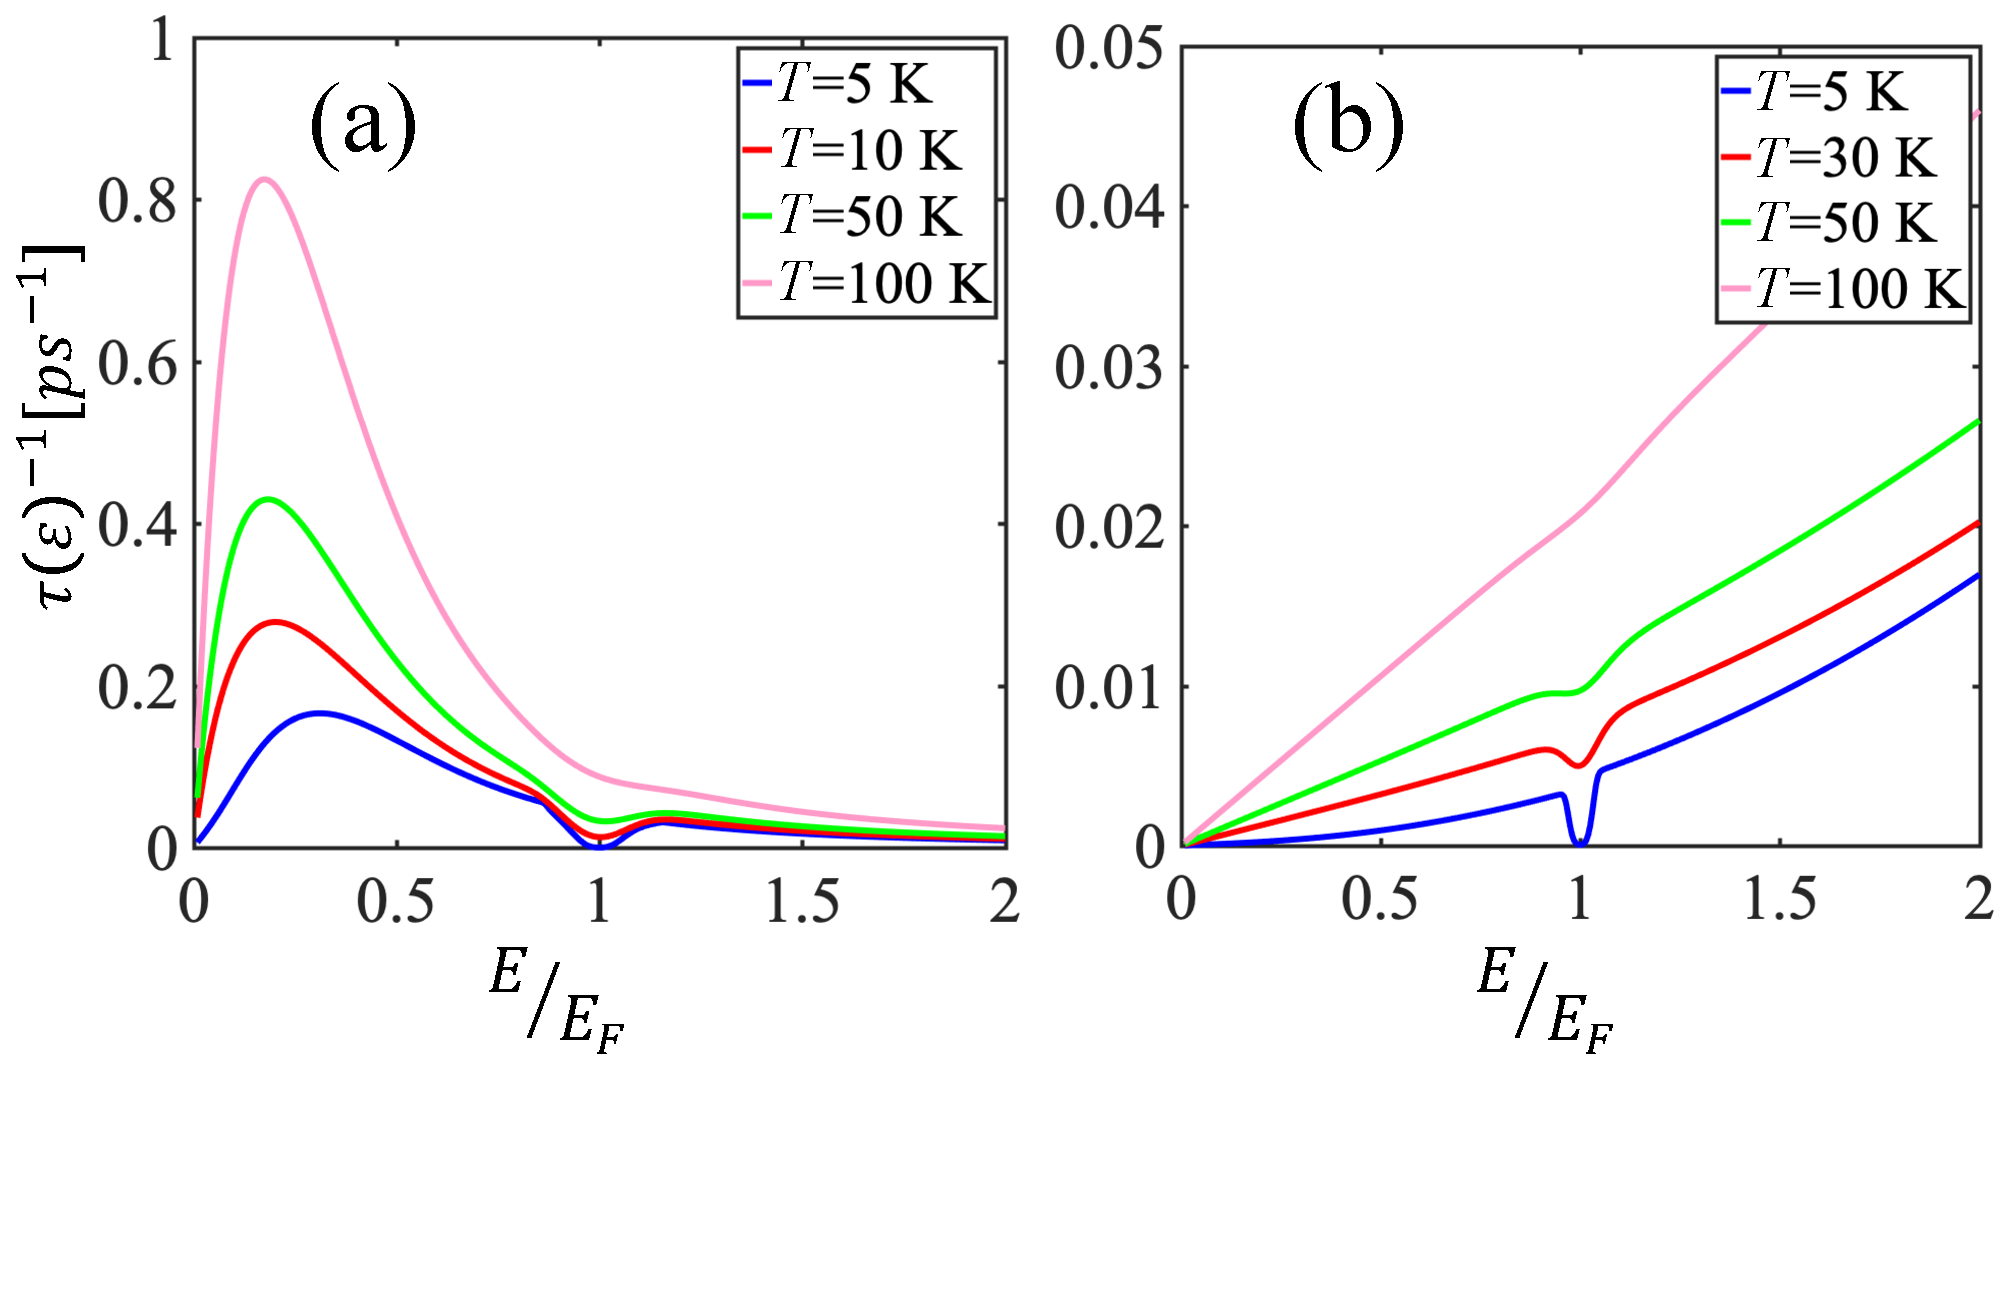
\includegraphics[width=0.79\textwidth]{Fig/Ch6/Fig3.pdf}
    \caption[Energy-dependent inverse relaxation time]{Energy-dependent inverse relaxation time of electrons in the (a) single-bogolon (emission and absorption) processes, and (b) phonon-assisted processes at different temperatures. In panel (a), $n_c=10^{11}$ cm$^{-2}$ and thus $s\approx 7\times 10^6$~cm/s. The figure is taken from~\cite{Sun:2019aa}.}
    \label{fig:CH6_3}
\end{figure}
%
%
%
Figure~\ref{fig:CH6_3} shows the inverse energy-dependent relaxation time as a function of energy for different temperatures.
We compare here the bogolon-mediated scattering with the acoustic phonon-assisted relaxation under certain conditions~\footnote{The formulas for phonons are taken from \cite{Hwang:2008aa} with the following parameters: graphene mass density $\rho=7.6\times 10^{-8}$~g$/$cm$^2$, phonon velocity $v_{ph}=2\times 10^6$~cm/s, deformation potential $D=6.8$~eV from \cite{Kaasbjerg:2012aa}, and electron density $n=10^{12}$~cm$^{-2}$.}.
%
We find some similarities between the bogolon- and phonon-mediated processes. In both cases, the inverse lifetime grows with increasing temperature due to the increase of the number of fermions and bosons (bogolons or phonons) in the system.
We also observe low-temperature dips at the Fermi energy, which are due to a sharpening of the Fermi surface.

Despite these similarities, there is a fundamental difference between the two principal channels of scattering, originating from the mechanisms of electron--phonon and electron--bogolon interaction.
The former derives from the crystal lattice deformation potential theory, while the latter has an electric nature and the matrix element contains the Coulomb interaction term.

%
%
%
\begin{figure}[ht]
\centering
    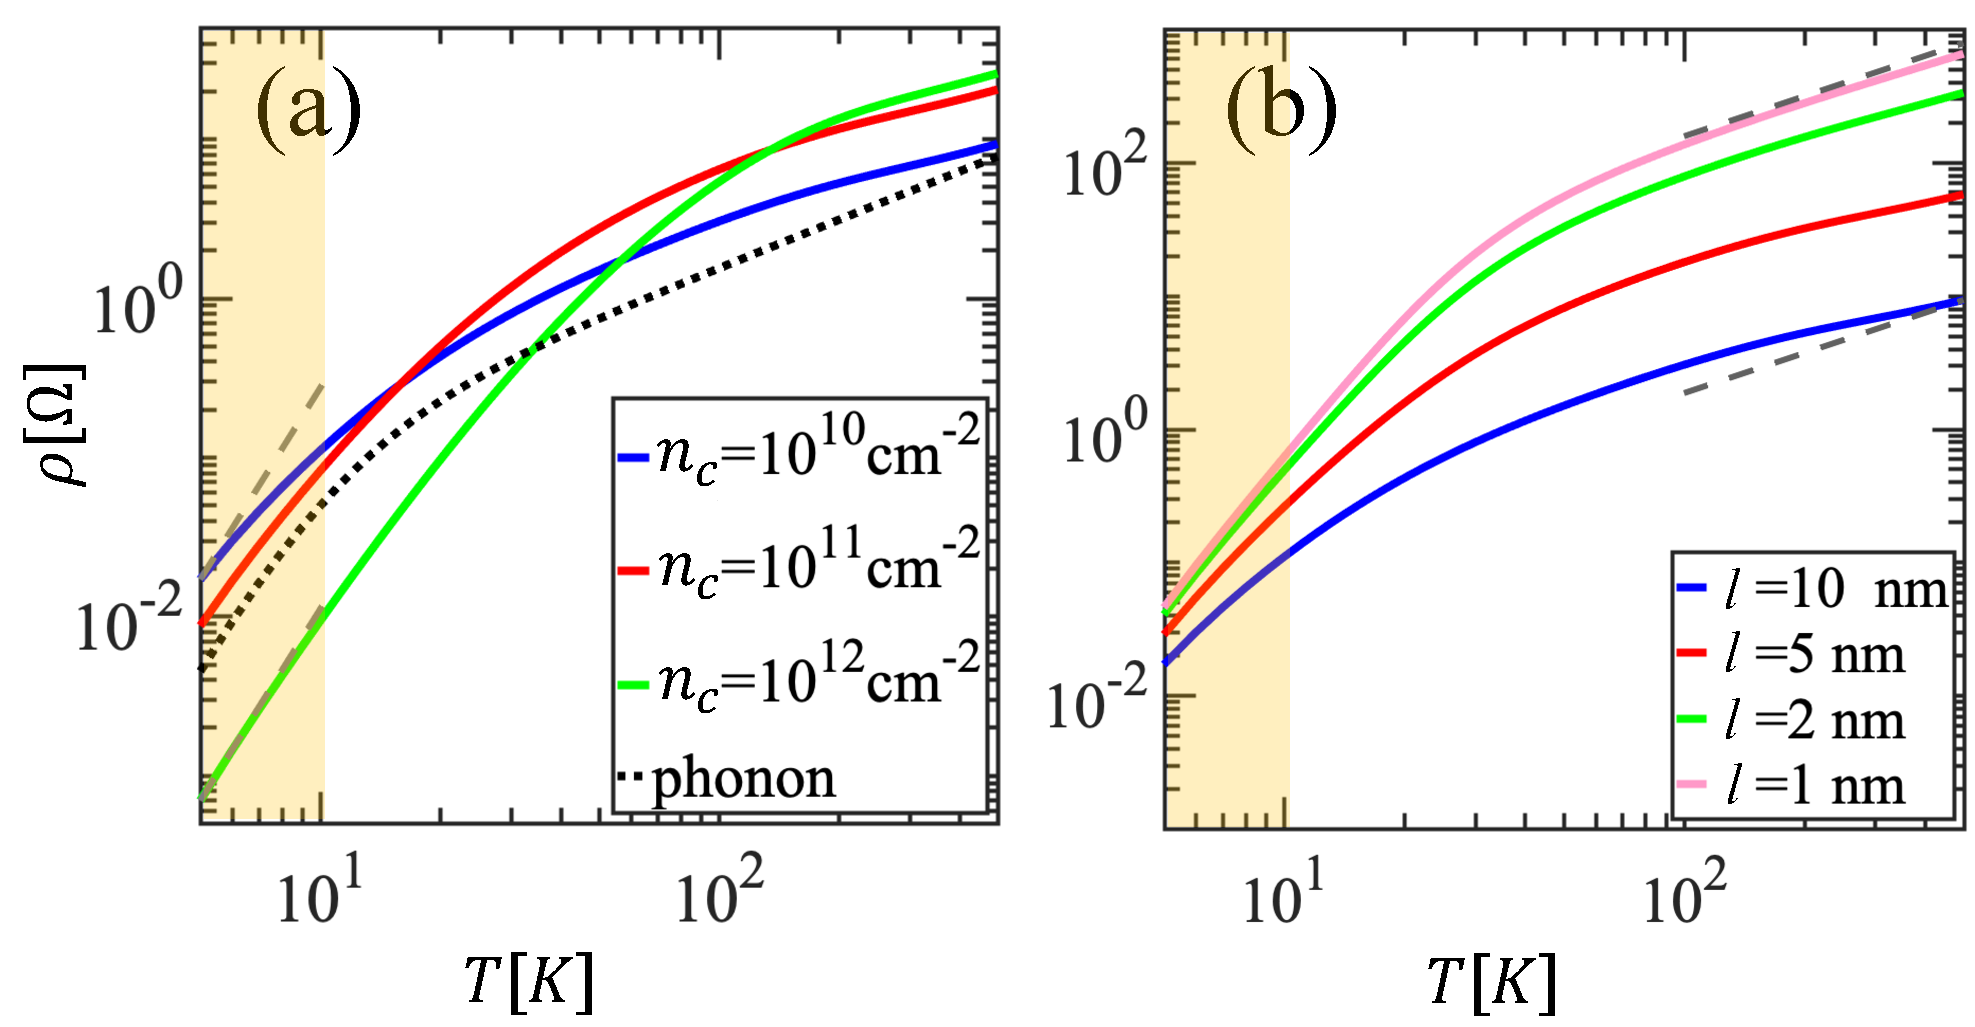
\includegraphics[width=0.79\textwidth]{Fig/Ch6/Fig4.pdf}
    \caption[Temperature-dependent bogolon-mediated resistivity]{Bogolon-mediated resistivity of graphene as a function of temperature for (a) different particle densities in condensate $n_c$ at $l=10$ nm, and for (b) different interlayer distances $l$ at $n_c=10^{10}$~cm$^{-2}$.
    The dashed grey lines stand for the low- and high-temperature analytics, indicating $\sim T^4$ and $\sim T$  behavior in (a) and (b) respectively.
    The black dotted line in (a) shows the phonon-mediated resistivity for comparison.
    The yellow-shaded regions highlight the temperature regime in which the condensation of indirect excitons in GaAs structures was experimentally reported. The figure is taken from~\cite{Sun:2019aa}.}
    \label{fig:CH6_4}
\end{figure}
%
%
%

Figure~\ref{fig:CH6_4} demonstrates the behavior of graphene resistivity as a function of temperature for different condensate densities and interlayer spacings.
We also compare this with the phonon-mediated resistivity.
All the curves show $\sim T^4$ dependence at low temperatures and $\sim T$ dependence at high temperatures.
Consequently, the primary behavior of resistivity is deceptively similar to the phonon-assisted case, as reported in~\cite{Hwang:2008aa}.
In the case of bogolons, different $n_c$ affect the sound velocity, and the Bloch--Gr\"{u}neisen temperature changes accordingly: $T_{BG} \approx 54$, $190$, and $540$~K for densities $n_c=10^{10}$, $10^{11}$, and $10^{12}$~cm$^{-2}$, respectively.
This is the reason why we obtain a better agreement between the numerical results and the $T^4$-analytics in the high-density regime.
Further, Fig.~\ref{fig:CH6_4}(b) shows that by decreasing $l$, we can increase the Coulomb interaction strength, thereby increasing the resistivity of graphene.

It should be noted that the parameters of a GaAs-based material were considered here.
Indirect excitons in such materials only condense at temperatures less than $10$ K (yellow regions in Fig.~\ref{fig:CH6_4}); however, a higher $T_c$, for which we predict a linear temperature dependence of resistivity, might be achieved in other materials or systems.
For example, the critical temperature for degenerate exciton Bose gas can possibly reach $\sim 100$~K in MoS$_2$~\cite{Fogler:2014aa}.
Another potential candidate is exciton-polaritons, where quasi-condensation has been reported even at room temperature~\cite{Lerario:2017aa}, even though in this situation one needs to consider the non-equilibrium physics which need to be investigated in the future.

%
% ------------------------------------
%
%\subsection{Conclusion}
%We have studied the finite--temperature electron conductivity in graphene, coupled with a two-dimensional dipolar exciton gas via the Coulomb interaction.
%We have calculated the energy--dependent relaxation time of electrons, accompanied by the emission and absorption of a Bogoliubov excitation.
%We have further calculated the resistivity of graphene in this hybrid Bose-Fermi system and showed that bogolon-mediated scattering not only gives a significant correction to the phonon-assisted relaxation but it prevails, given specific system geometry and temperatures.
%We believe the reported results can be used to design new types of graphene-based hybrid systems.

%
% ------------------------------------
\section{Metal Case}
In this section, we consider a system consisting of a 2DEG with a parabolic dispersion of electrons and a layer of Bose-condensed exciton gas~\cite{Butov:2003aa,Fogler:2014aa,Butov:2017aa}.
\subsection{Single-bogolon scattering}
To investigate the principal $T$-dependence of single bogolon mediated resistivity at low temperatures, we follow the routine discussed in Section~\ref{sec:low} by writing the Boltzmann equation
%
\begin{eqnarray}
\label{CH7_Eq1}
e_0\textbf{E}\cdot\frac{\partial f}{\hbar\partial \textbf{p}}=I\{f\},
\end{eqnarray}
%
where $f$ is the electron distribution function, $\mathbf{p}$ is the wave vector, $\mathbf{E}$ is an external electric field, and $I\{f\}$ is the collision integral involving single-bogolon scattering processes, as shown in Fig.~\ref{fig:CH6_2}(a) and (b) (see Appendix~\ref{AP:CH7} for the explicit form of $I$ and other details of derivation).
For relatively weak electric fields, we apply Eq.~\ref{CH6_f} to express the function $f$,
%
% \begin{eqnarray}
% f=f^0(\varepsilon_p)-\left(-\frac{\partial f^0}{\partial\varepsilon_p}\right)\phi_\textbf{p},
% \end{eqnarray}
%
% where $p\equiv\abs{\mathbf{p}}$, $f^0(\varepsilon_p)$ is the Fermi-Dirac distribution.
% The function $\phi_\textbf{p}$ is the change in energy of the electron due to the applied field.
% Without the loss of generality, we put this electric field to be directed along the $x$-axis and use the ansatz
%
where for the 2DEG case we express the term $f^{\left(1\right)}_\mathbf{p}$ as
\begin{equation}
\label{CH7_EqAnsatz}
\phi_\textbf{p}= (e_0E_x)(\hbar m^{-1}p_x)\tau(\varepsilon_p),
\end{equation}
%
where $m$ is the effective electron mass in the 2DEG and $\tau(\varepsilon_p)$ is the relaxation time.
The factor $e_0E_x$ is the force acting on the electron while $\hbar m^{-1}p_x$ is the electron velocity.
The function $\phi_\mathbf{p}$ therefore gives the work done by the electric field on the electron during time $\tau(\varepsilon_p)$.

Using Eqs.~\eqref{CH7_Eq1} and~\eqref{CH7_EqAnsatz}, we find the average value of the scattering time (see Appendix~\ref{AP:CH7}) and then the single bogolon mediated resistivity, which is
%
\begin{eqnarray}
\label{CH7_rho1bgen}
\rho^{(1)}=\frac{\pi\hbar^3\xi_I^2}{e_0^2ME_F}\sum_{n=0}^\infty\frac{(-2)^nl^n\gamma_n}{n!(\hbar s)^{n+4}}(k_BT)^{n+4},
\end{eqnarray}
%
where $\xi_I= e_0^2d\sqrt{n_c}/2\epsilon$, $E_F$ is the Fermi energy, $\gamma_n=(n+3)!\zeta(n+3)/[(2\pi)^2k_BT_\textrm{BG}]$, $T_\textrm{BG}=2\hbar sk_F/k_B$ is the Bloch--Gr\"{u}neisen temperature with $k_F$ the Fermi wave vector, $k_B$ the Boltzmann constant, and $\zeta(x)$ the Riemann zeta function.
The leading term in Eq.~\eqref{CH7_rho1bgen}, if $T\ll T_\textrm{BG}$, reads
%
\begin{eqnarray}
\label{CH7_rho1b}
\rho^{(1)}\approx\frac{\pi\hbar^3\xi_I^2}{e_0^2ME_F}\frac{3!\zeta(3)}{(2\pi)^2k_BT_\textrm{BG}}\left(\frac{k_BT}{\hbar s}\right)^4,
\end{eqnarray}
%
and hence the single bogolon resistivity behaves as $\rho^{(1)}\propto T^4$ at low temperatures.

%
% --------------------------------------------
%
\subsection{Double bogolon scattering}
Double bogolon resistivity can also be derived from Eq.~\eqref{CH7_Eq1}. The collision integral now expresses the net scattering into a state with momentum $\hbar\mathbf{p}$, involving a pair of bogolons, as shown in Fig.~\ref{fig:CH6_2}(c--f) (see also Appendix~\ref{AP:CH7}).
After some delicate derivations we find
%
\begin{eqnarray}
\label{CH7_rho2bmain}
\rho^{(2)}=\frac{M^2s^2}{8\pi^2e_0^2m^3v_F^5}\int\limits_{L^{-1}}^\infty\frac{k^2g_k^2dk}{\sinh^2\left[\frac{\hbar sk}{2k_BT}\right]}\ln(kL),
\end{eqnarray}
%
where $v_F$ is the Fermi velocity.
To derive Eq.~\eqref{CH7_rho2bmain}, we used the approximation $v_F\gg s$ and introduced the infrared cut-off $L^{-1}$ for the wave vector integrals, which is necessary for convergence.
The physical meaning of this cut-off is the absence of fluctuations with wavelengths larger than $L$.
The cut-off can also be related to the critical temperature of the BEC in a finite trap of length $L$~\cite{Bagnato:1991aa}.
Indeed, BEC cannot form in infinite homogeneous 2D systems at finite temperatures~\cite{Hohenberg:1967aa}, and thus a trapping with a characteristic size of $L$ is required~\cite{Butov:2017aa}.

We can further extract the temperature dependencies for the two limits (see Appendix~\ref{AP:CH7}).
At low temperatures $T\ll T_\textrm{BG}$,
%
\begin{eqnarray}
\label{CH7_rho2b}
\rho^{(2)}\approx\frac{s^2e_0^2d^2}{2v_F^5\epsilon^2}\left(\frac{T}{T_\textrm{BG}}\right)^3\frac{\pi}{6(2l)^3}\ln \left(\frac{L}{2l}\right),
\end{eqnarray}
%
while at high temperatures $T\gg T_\textrm{BG}$,
%
\begin{eqnarray}
\label{CH7_highT}
\rho^{(2)}\approx\frac{s^2e_0^2d^2}{2v_F^5\epsilon^2}\left(\frac{T}{T_\textrm{BG}}\right)^2\frac{1}{(2l)^3}\ln \left(\frac{L}{2l}\right).
\end{eqnarray}
%
%
%

%
%
%
\begin{figure}[ht]
\centering
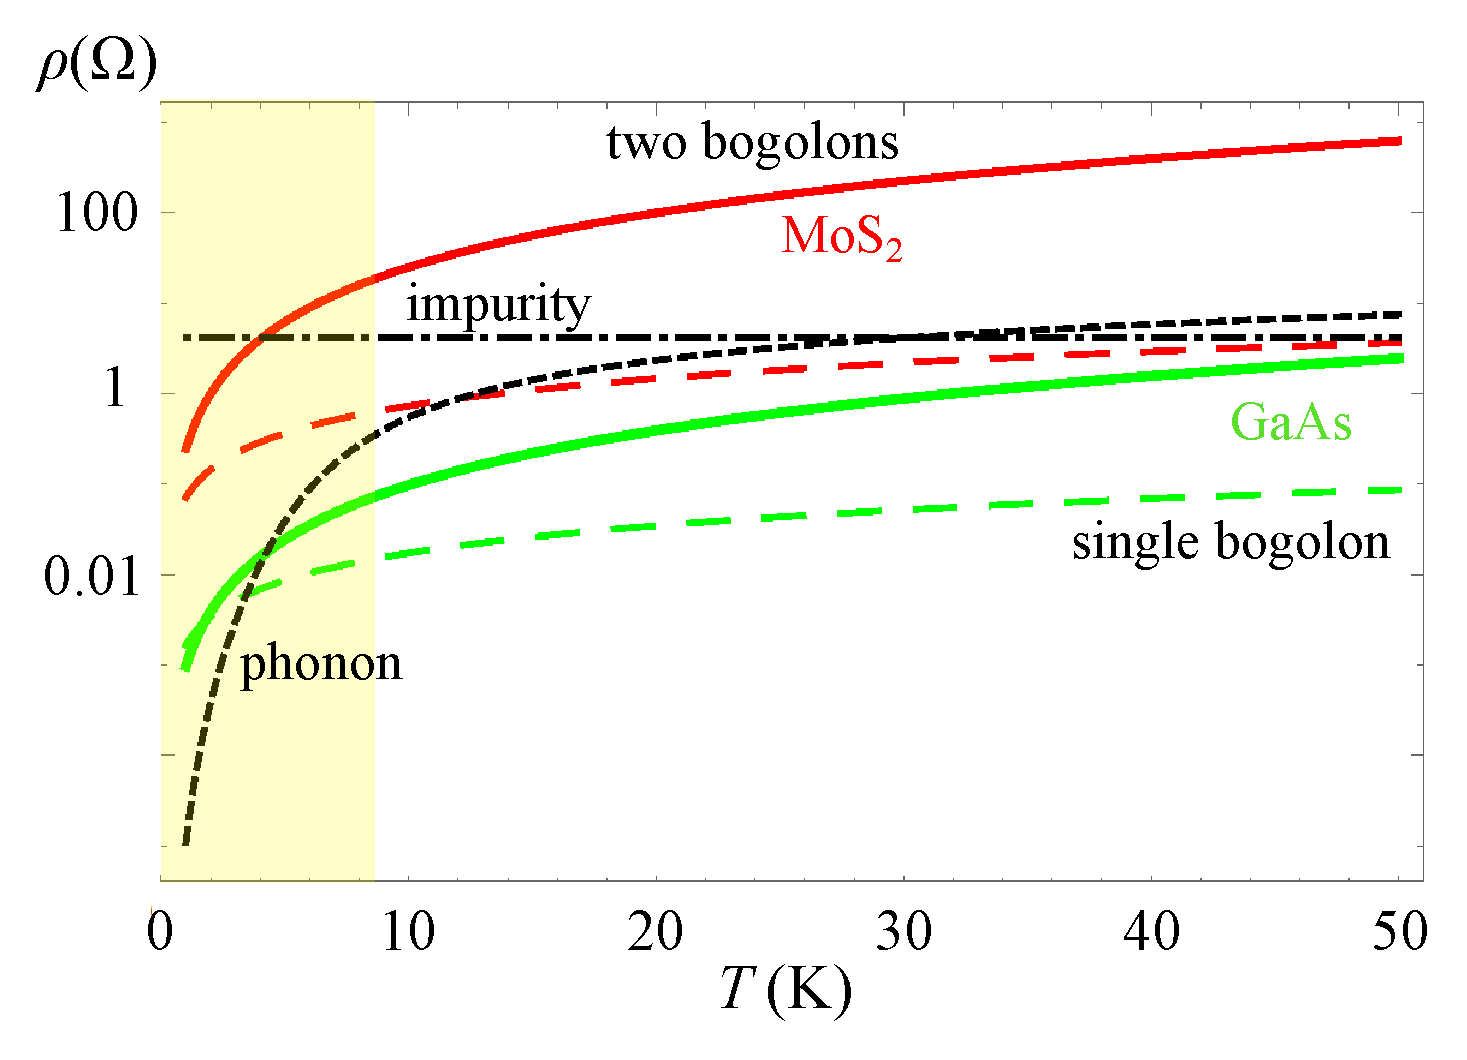
\includegraphics[width=0.65\textwidth]{Fig/Ch6/Fig1ER.pdf}
\caption[Temperature-dependent resistivity of $\textrm{MoS}_2$ and GaAs]{Resistivity as a function of temperature for MoS$_2$ (red) and GaAs (green) exciton condensates.
Colored solid and dashed curves stand for the double-bogolon and single-bogolon contributions, respectively.
Black dash-dotted and dashed curves show the impurity and phonon contributions, respectively. We set $n_e=10^{13}$~cm$^{-2}$ and $n_c=10^9$~cm$^{-2}$. The figure is taken from~\cite{Villegas:2019aa}.}
\label{CH7_Fig3}
\end{figure}
%
%
%

%
% ------------------------------------------
%
\subsection{Discussion}
Compared to Eq.~\eqref{CH7_rho1b}, we conclude that the double-bogolon process should dominate over the single-bogolon process at very low temperatures.
However, in this range, scattering due to impurities is usually the strongest, which hinders the possibility to observe low-temperature asymptotics.
%
Figure~\ref{CH7_Fig3} shows the temperature behavior of different principal contributions to resistivity. In order to compare bogolon-mediated scattering with the scattering from phonons and impurities, we employed the theoretical and experimental results reported elsewhere~\cite{Kawamura:1992aa, Macleod:2009aa, Min:2012aa,Mendez:1984aa,Hirakawa:1986aa,Gold:1990aa}
and the parameters characteristic of a 2DEG in GaAs and excitons in both GaAs and MoS$_2$ materials\footnote{The values of the parameters were taken from~\cite{Kaasbjerg:2013aa,Basu:1980aa,Mair:1997pt} as follows.
Dielectric constants: $\epsilon_\textrm{GaAs}=12.5\epsilon_0$, $\epsilon_{\textrm{MoS}_2}=4.89\epsilon_0$; effective electron masses ($m_0$ is the bare electron mass): $m_\textrm{GaAs}=0.067m_0$, $m_{\textrm{MoS}_2}=0.47m_0$; exciton masses: $M_\textrm{GaAs}=0.517m_0$, $M_{\textrm{MoS}_2}=0.499m_0$; exciton sizes: $d_\textrm{GaAs}=10.0$ nm, $d_{\textrm{MoS}_2}=3.5$ nm; deformation potential: $D_\textrm{GaAs}=12$ eV.
}.

Figure~\ref{CH7_Fig3} shows the dependence of resistivity on temperature in the range$1-50$~K.
We set the concentration of impurities as $n_i=10^9$ cm$^{-2}$, which is attainable in high-quality $\textrm{GaAs}$ 2DEG~\cite{Hwang:2008ab,Manfra:2014aa}.
The yellow-shaded region highlights the low-temperature regime $T\ll T_\textrm{BG}$, where for both $\textrm{GaAs}$ and $\textrm{MoS}_2$ materials, $T_\textrm{BG}\approx 80$~K.
In this regime, the impurity scattering dominates even in high-quality $\textrm{GaAs}$ 2DEG;
however, when $T>14$~K we see that the double-bogolon scattering contribution to the resistivity can become an order of magnitude larger than all other contributions, if the double QW is made of $\textrm{MoS}_2$ material.
Scattering processes from impurities, phonons, and single bogolons have comparable contributions in the temperature range $20-50$~K.
The critical temperature of exciton quasi-condensation (or the formation of a degenerate Bose gas) in $\textrm{GaAs}$ has been reported to be around $T_c\sim 1-7$~K~\cite{Butov:2003aa}, and it is predicted to reach $T_c\sim 100$~K in $\textrm{MoS}_2$~\cite{Fogler:2014aa}.
We can alternatively put the structure from Fig.~\ref{fig:Ch6_1} in a microcavity, and instead of indirect excitons consider exciton-polaritons---for this, the same treatment is possible except for a different effective mass and the appearance of the Hopfield coefficients. In such a scenario, degenerate Bose gas (quasi-condensation or superfluidity) has been reported even at room temperature~\cite{Lerario:2017aa}.
One can also consider 2DEG in graphene instead of GaAs, where the scattering from impurities is suppressed and mobility is high.

In the conventional approach to hybrid 2DEG--BEC systems, the double-bogolon interaction, Eq.~\eqref{CH6_eq.5-b}, has been disregarded as it relates to second-order perturbation theory in fluctuations above the macroscopically-occupied ground state.
Figure~\ref{CH7_Fig3} demonstrates that this widespread approximation is not valid in the context of the  exciton condensates in MoS$_2$ material.
For GaAs exciton layers, the impurity is dominant for temperatures from $T\sim0-3$~K, at which the condensates can exist.
Hence, we will focus on MoS$_2$ in what follows.

%
%
%
\begin{figure}[ht]
\centering
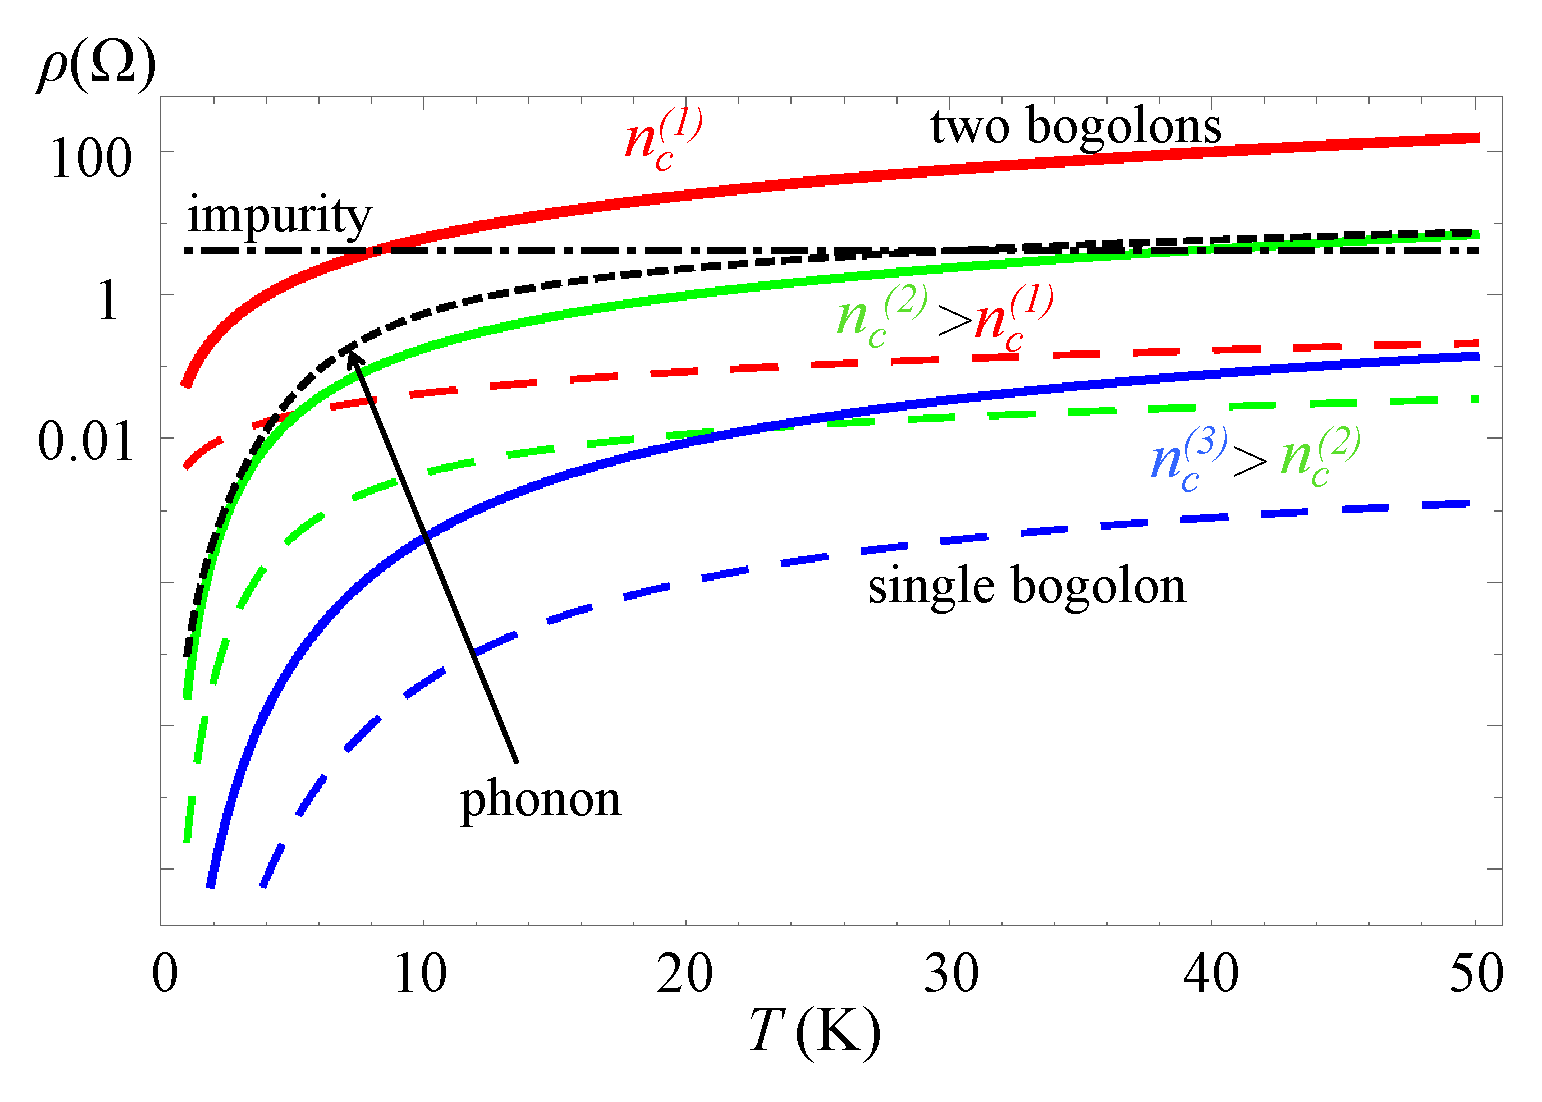
\includegraphics[width=0.65\textwidth]{Fig/Ch6/Fig2ER.pdf}
\caption[Temperature-dependent resistivity with different condensate densities]{Temperature dependence of resistivity for various MoS$_2$ condensate densities: $n_c=10^8$~cm$^{-2}$ (red), $n_c=10^{10}$~cm$^{-2}$ (green), and $n_c=10^{11}$~
cm$^{-2}$ (blue).
The corresponding Bloch--Gr\"{u}neisen temperatures are $T\sim17$, $174$, and $549$~K, respectively. Black dash-dotted and dashed curves show the impurity and phonon contributions, respectively.
The electron density is fixed at $n_e=5\times10^{12}$~cm$^{-2}$. The figure is taken from~\cite{Villegas:2019aa}.}
\label{CH7_Fig4}
\end{figure}
%
%
%

Figure~\ref{CH7_Fig4} demonstrates the dependence of resistivity on condensate densities in the MoS$_2$-based exciton layer.
One can see that both single- and double-bogolon contributions increase as the condensate density decreases at relatively low temperatures (blue to green, green to red).
Such a tendency can be understood from Eqs.~\eqref{CH7_rho1b} and~\eqref{CH7_rho2b}, giving $\rho^{(1)}\sim \xi_I^2/(T_\textrm{BG}s^4)\sim n_c^{-1.5}$ and $\rho^{(2)}\sim s^2/T^3_\textrm{BG}\sim n_c^{-0.5}$.
Note that a similar behavior in the single-bogolon case happens in exciton BEC--graphene structures~\cite{Sun:2019aa}.
At $T\gg T_\textrm{BG}$ though, $\rho^{(2)}$ becomes $n_c$-independent, as follows from Eq.~\eqref{CH7_highT}; this could be seen by the red, green, and blue solid curves in Fig.~\ref{CH7_Fig4} starting to approach each other at higher temperatures.
We further note that the BEC-related screening from impurity and phonon processes has no significant effect, and so we plotted only two related curves.

Here we emphasize that these observations are valid as long as $n_c$ is macroscopically large, for the following two reasons.
%There are two reasons for this limitation.
First, in our calculations, we assume that the bogolon dispersion is linear (see Appendix~\ref{AP:CH7}), which only remains valid for $n_c\gtrsim 10^8$ cm$^{-2}$. %
Second, even if this assumption could be relaxed, we note that replacing the exciton field operator through $\Phi_\mathbf{R}=\sqrt{n_c}+\varphi_\mathbf{R}$, where $n_c$ is treated as an ordinary complex number instead of an operator, represents a mean field approach which is an essential ingredient of the Bogoliubov theory. %It is valid if $n_c$ is macroscopically occupied and the fluctuations above it are small.
Thus, we cannot expand our conclusions to the $n_c\rightarrow 0$ limit.
Despite this, we expect that in this limit, the bogolon contribution should vanish and be replaced by the bare exciton contribution, as dictated by $u_{\mathbf{p}}=1$ and $v_{\mathbf{p}}=0$ in Eqs. \eqref{CH6_eq.5-a} and~\eqref{CH6_eq.5-b}.

The dependence of resistivity on the separation between layers $l$ turns out rather strong, as expected, while the dependence on sample size $L$ (for double-bogolon scattering, where we introduced the infrared cut-off) is weak~(see Appendix~\ref{AP:CH7}).
This allows us to optimize sample design by varying $l$.

%
%
%
\begin{figure}[ht]
\centering
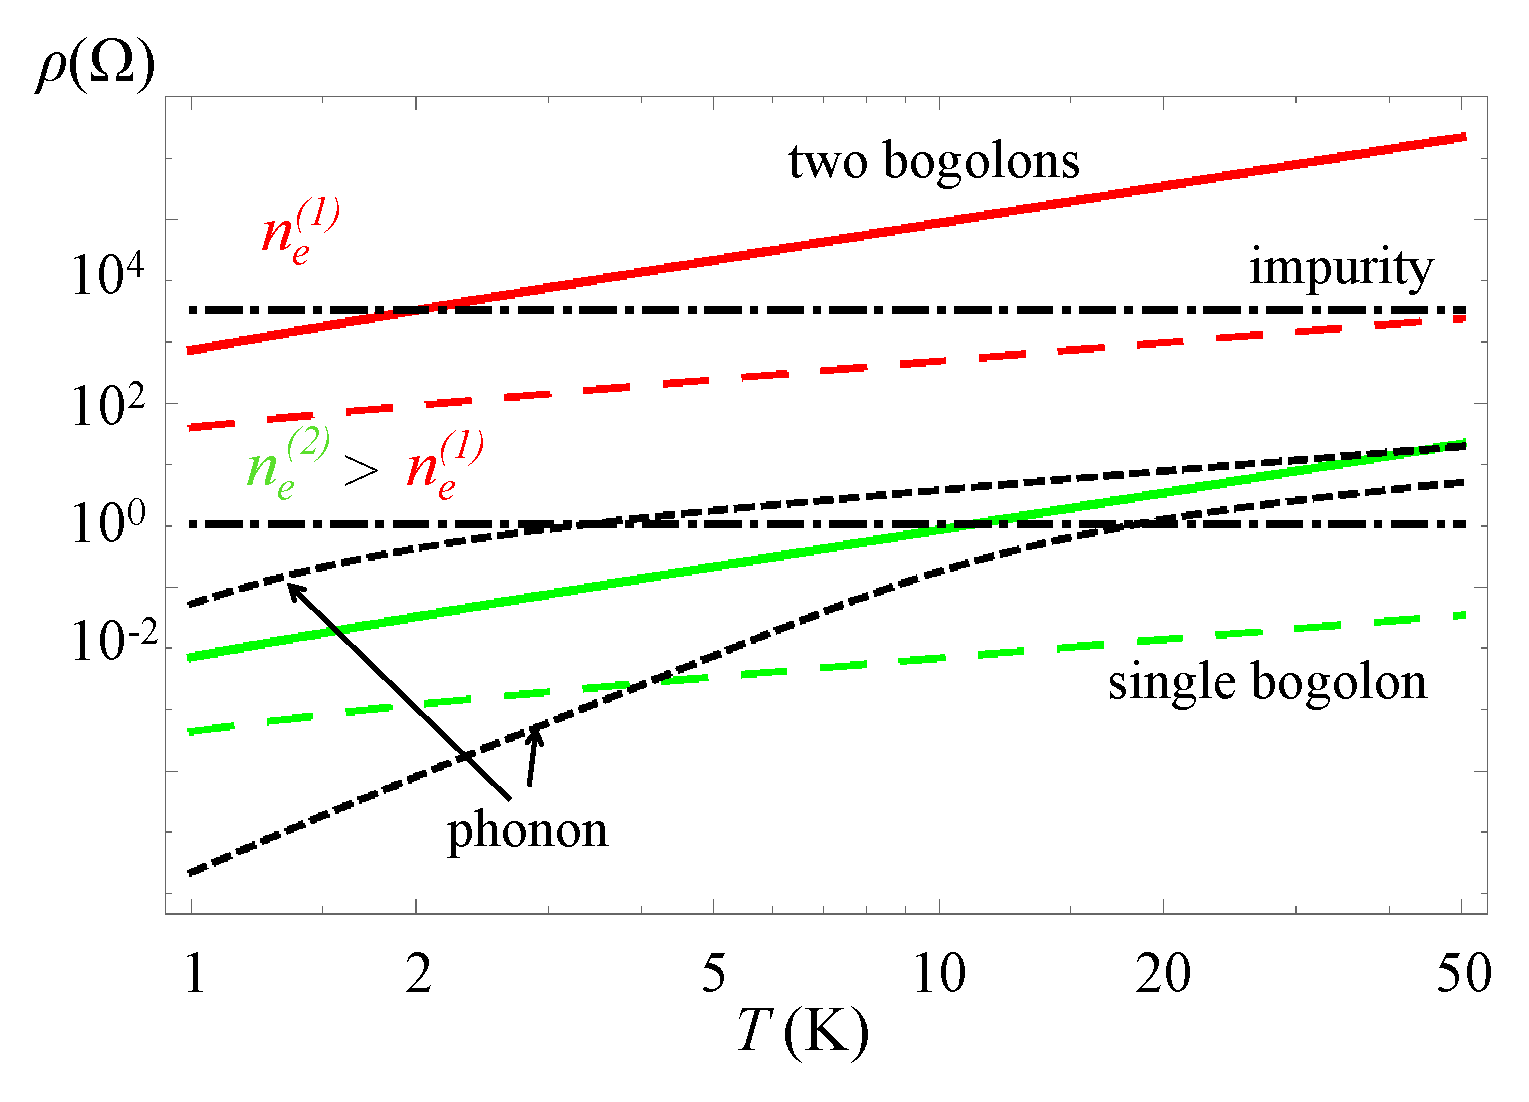
\includegraphics[width=0.65\textwidth]{Fig/Ch6/Fig3ER.pdf}
\caption[Resistivities of single- and double-bogolon processes]{Temperature dependence of single-bogolon (dashed colored) and double-bogolon (solid colored) resistivities at different electron densities: $n_e=10^{11}$ (red) and $n_e=10^{13}$~cm$^{-2}$ (green). The corresponding Bloch--Gr\"{u}neisen temperatures are $T\sim2$ and $25$~K, respectively.
Black dash-dotted and dashed curves show the impurity and phonon contributions, respectively.
The density of the MoS$_2$ condensate is $n_c=10^8$~cm$^{-2}$. The figure is taken from~\cite{Villegas:2019aa}.}
\label{CH7_Fig5}
\end{figure}
%
%
%

The bogolon, impurity, and phonon-mediated resistivities all depend on the density of charge carriers in the 2DEG (see Fig.~\ref{CH7_Fig5}), and therefore generally decrease with an increase of $n_e$.
However, they do so at different rates.
For example, at $n_e=10^{13}$~cm$^{-2}$, impurity-induced scattering is dominant in the temperature range $T\sim 0-20$~K, while both the double-bogolon- and phonon-induced scattering become dominant (with comparable contributions) at $T\sim 20-50$~K.
At the lower density $n_e=10^{11}$~cm$^{-2}$, double-bogolon scattering starts to give the largest contribution at $T\gtrsim 5$~K, even reaching two orders of magnitude greater than the impurity contribution at $50$~K.

The dominance of the double-bogolon channel over the single-bogolon scattering in the MoS$_2$ exciton layer can be understood from an analysis of the matrix elements in the Fermi golden rule.
In the single-bogolon case, there appears a small factor $(u_\mathbf{p}+v_{-\mathbf{p}})\sim\sqrt{1+A^2}-A$, where $A=(Ms)/(\hbar \lambda)$ (see Appendix~\ref{AP:CH7}).
In other words, $(u_\mathbf{p}+v_{-\mathbf{p}})\sim(p\xi)^2\ll 1$.
In particular, in MoS$_2$, this factor is sufficiently small to compensate the large value of $\sqrt{n_c}$.
In contrast, there is no such cancellation effect in the double-bogolon terms, where there appears the product $u_\textbf{p}v_\textbf{p}\sim (p\xi)^{-1}\gg 1$ instead of $u_\mathbf{p}+v_{-\mathbf{p}}$.
Here we can compare with phonon scattering, where this cancellation effect does not take place, so that single-phonon scattering has larger contribution than double-phonon scattering.
This argument illustrates the difference between bogolon and phonon-assisted scattering, which is due to the difference in the origin of Coulomb interaction between the particles.

Experimentally, it might be difficult to resolve all the different contributions to the total resistivity, especially at low temperatures.
However, using the analytical formula Eq.~(\ref{CH7_highT}), we predict that the high-temperature resistivity should behave as $\rho\sim T^2$, if the double-bogolon scattering gives the dominant contribution.
This is in contrast to phonons giving $\rho\sim T$, and impurities with nearly absent $T$-dependence.

%What can we say about the electron pairing in such a hybrid 2DEG-BEC system below $T_c$?
%For any metal in the normal (not superconducting) state, the strength of electron-phonon interaction is responsible for the resistivity due to the scattering.
%Obviously, the stronger the interaction strength (which is mostly determined by the matrix element of interaction), the larger is the resistivity.
%In the superconducting phase, the electron pairing is also mediated by the interaction with phonons (or bogolons~\cite{Laussy:2010aa}).
%Indeed, there enters the same matrix element of the electron-phonon interaction. The bigger it is, the larger the superconducting gap opens, which means a robust superconductivity.
%The critical temperature is also determined by the strength of the electron-phonon (bogolon) interaction. It makes us suppose that \textit{bad} conductors in the normal phase are \textit{good} superconductors and suggest an alternative mechanism of high-temperature pair-of-bogolons--mediated superconductivity.

\section{Summary}
In this chapter, we have studied the transport of electrons in graphene and 2D metals coupled with a 2D Bose-condensed dipolar exciton gas via Coulomb interaction.

In the graphene case, we calculated the energy-dependent relaxation time of electrons, accompanied by the emission and absorption of a Bogoliubov excitation.
We further showed that bogolon-mediated scattering not only gives a significant correction to the phonon-assisted relaxation, but it also prevails given specific system geometry and temperatures.

In the 2DEG case, we calculated the resistivity by extending the Bloch--Gr\"{u}neisen approach and provided analytical formulas for the single- and double-bogolon scattering channels. We discovered that double-bogolon scattering becomes the dominant mechanism in hybrid systems in a certain range of temperatures.
%Furthermore, we suggested an alternative way of electron pairing, as mediated by a pair of bogolons.
%
% \subsection{Conclusion}
% We have studied the finite--temperature electron conductivity in graphene, coupled with a two-dimensional dipolar exciton gas via the Coulomb interaction.
% We have calculated the energy--dependent relaxation time of electrons, accompanied by the emission and absorption of a Bogoliubov excitation.
% We have further calculated the resistivity of graphene in this hybrid Bose-Fermi system and showed that bogolon-mediated scattering not only gives a significant correction to the phonon-assisted relaxation but it prevails, given specific system geometry and temperatures.
% We believe the reported results can be used to design new types of graphene-based hybrid systems.
